\documentclass[12pt,a4paper]{report}
\usepackage[utf8]{inputenc}
\usepackage[english]{babel}
\usepackage{amsmath}
\usepackage{amsfonts}
\usepackage{amssymb}
\usepackage{amsmath}
\usepackage{graphicx}

\usepackage[object=vectorian]{pgfornament}
\usepackage{lipsum,tikz}
\usepackage{listing}

\usepackage{subfig}
\usepackage{hyperref}
\usepackage{chemformula}
\usepackage[object=vectorian]{pgfornament} %%  http://altermundus.com/pages/tkz/ornament/index.html
\usepackage[left=2cm,right=2cm,top=2cm,bottom=2cm]{geometry}
\usepackage{hyperref}

\newcommand{\sectionline}[2]{%
  \nointerlineskip \vspace{.5\baselineskip}\hspace{\fill}
  {\color{#1}
    \resizebox{0.5\linewidth}{2ex}
    {{%
    {\begin{tikzpicture}
    \node  (C) at (0,0) {};
    \node (D) at (9,0) {};
    \path (C) to [ornament=#2] (D);
    \end{tikzpicture}}}}}%
    \hspace{\fill}
    \par\nointerlineskip \vspace{.5\baselineskip}
  }



\usepackage{titlesec}
\newcommand{\sectionbreak}{\clearpage}



\begin{document}


\title{%
  \large The Weekly Progress Report \\
    }

\author{Ilia Kulikov}


\setcounter{chapter}{+1}
\maketitle

\section{This Week}
This week I solved eq. 1.1 numerically and saw that the finger grid problem solves trivially if the fingers are far away from each other. We were also working on the G-RISC report and on the electrochemistry paper together with Naitik and Anatoliy. Hopefully Anatoliy will send both files to Jan soon. For the battery project, a group in Mendeley was created, where all invited participants can add literature. Invited Naitik and Jan. Worked on the Hall manuscript. Installed cisco webex. I guess that is essential for seminars.\\
\subsection{Batteries}
\par \textbf{Plotting}: Almost all of the data is plotted by now. Now we need to plot the spin count versus potential for the waterfall plots. Sample 7 is the most interesting sample for that. Also we are having a closer look to the DiTS monomer in AN solution at different temperatures.\\
\par \textbf{5-line simulations}: DiTS monomer in solution shows a certain five-line signature (Fig. \ref{fig:dits_mono} for 273K). That signature is well described in the Eatons' paper on dinitroxide radicals. I think, we have two stable conformations of DiTS that yield this signature: Low-\textbf{J} and high-\textbf{J} conformation that can explains the apparent overlap of 3-line hyperfine and 5-line exchange structures in the spectrum. Naitik studied the 5-line spectra at different temperatures. He suggests that there are three stable conformations of the DiTS molecule.\\ 
A part of the signal in Fig.\ref{fig:dits_mono} is in saturation. The intense, three-line substructure is not in saturation, but the two inner lines are saturated. We have not discussed the saturation yet, but that might suggest that we may distinguish between at least two subsystems in DiTS.\\

The plotting plan now has now more comments. It also contains datasets, plots and the scripts with which the data was plotted. Latest plot so far is shown in Fig. \ref{fig:dits_temps}. This is the CW spectrum of a dry DiTS film during cooling downto 53K. The signal does not vanish downto 53K. We later saw a CW signal from DiTS on the pulsed spectrometer at even colder temperatures. Unfortunately we have not seen the echo so far.\\
\begin{verbatim}/EPR on Batteries/Project Planning/plotting_plan_100420_IK.ods
\end{verbatim}

\begin{figure} [!ht]

\begin{center}
       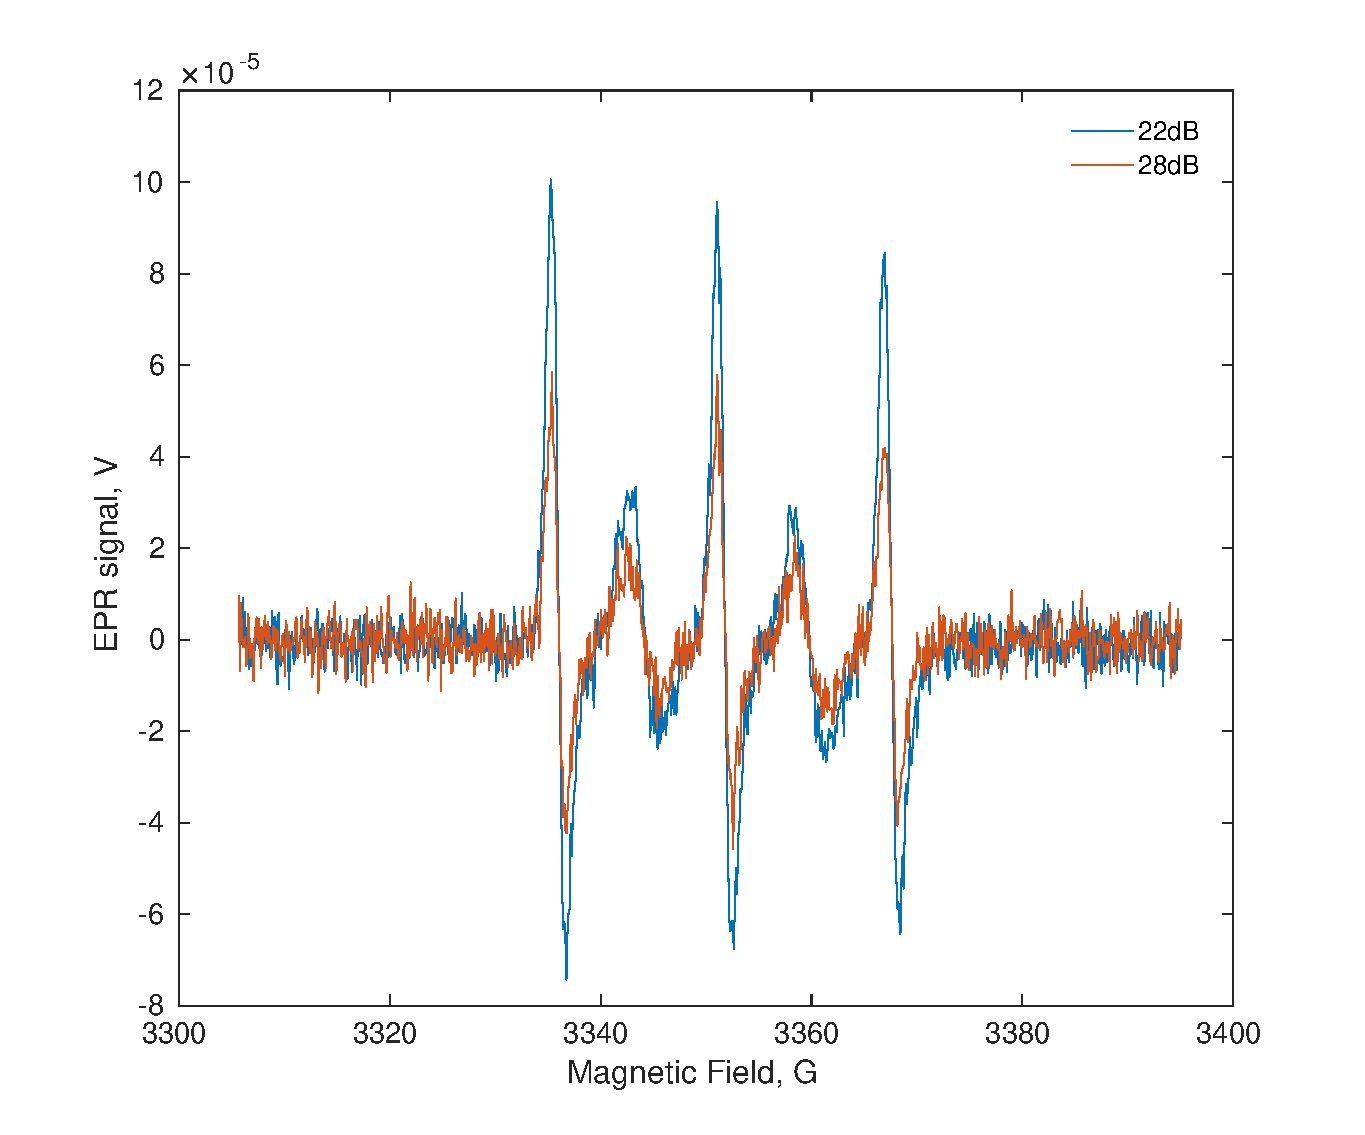
\includegraphics[width=1\textwidth]{./pics_200410/plt_40_DiTS_monomer_in_AN_sat.pdf}
       \end{center}
\caption{DiTS monomer in AN at 273K. The characteristic five-line strusture. Partial saturation of the signal.}
     \label{fig:dits_mono}
\end{figure}

\begin{figure} [!ht]

\begin{center}
       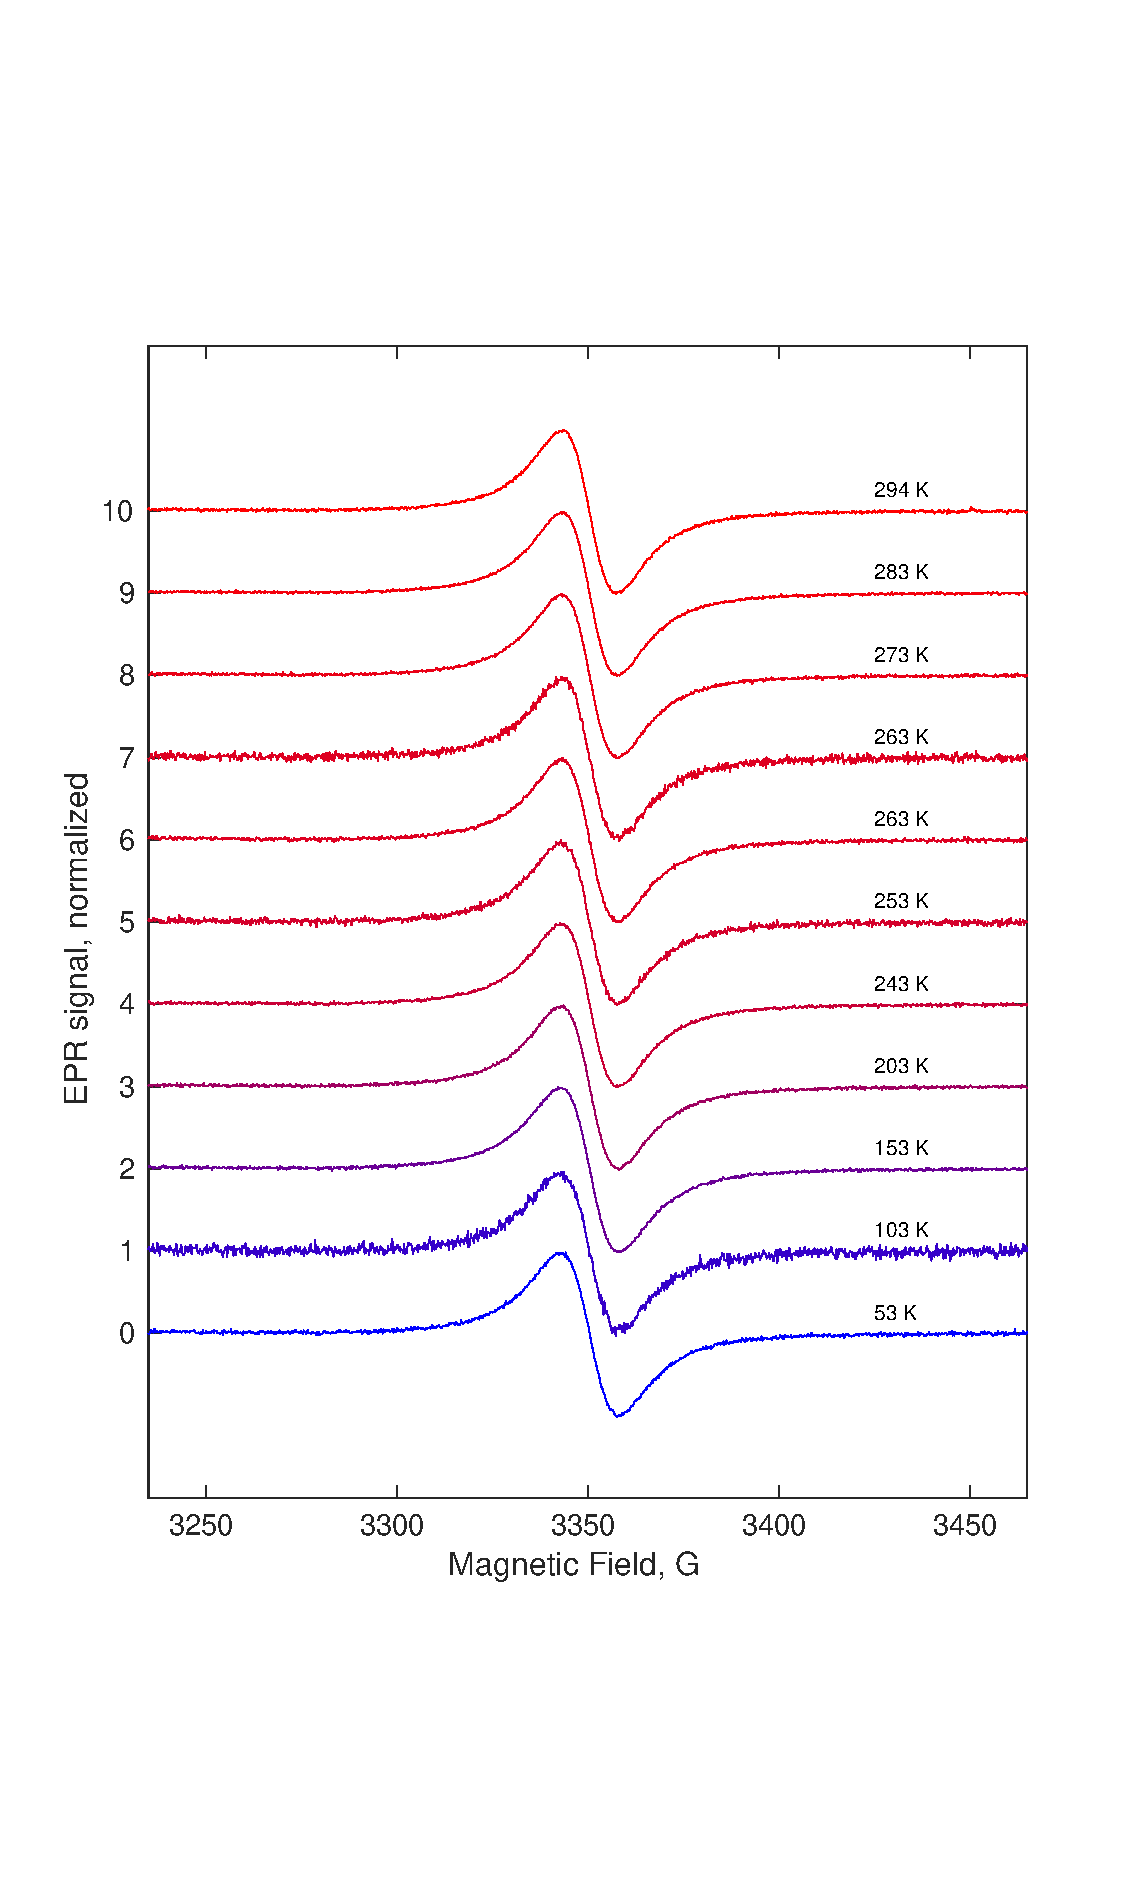
\includegraphics[width=1\textwidth]{./pics_200410/plt_38_S6_temp_series.pdf}
       \end{center}
\caption{Freezing of sample 6 in the framework of preparation for the pulsed measurements at low temperatures. }
     \label{fig:dits_temps}
\end{figure}

\subsection{Finger Grids}

\begin{figure} [!ht]
\begin{center}
       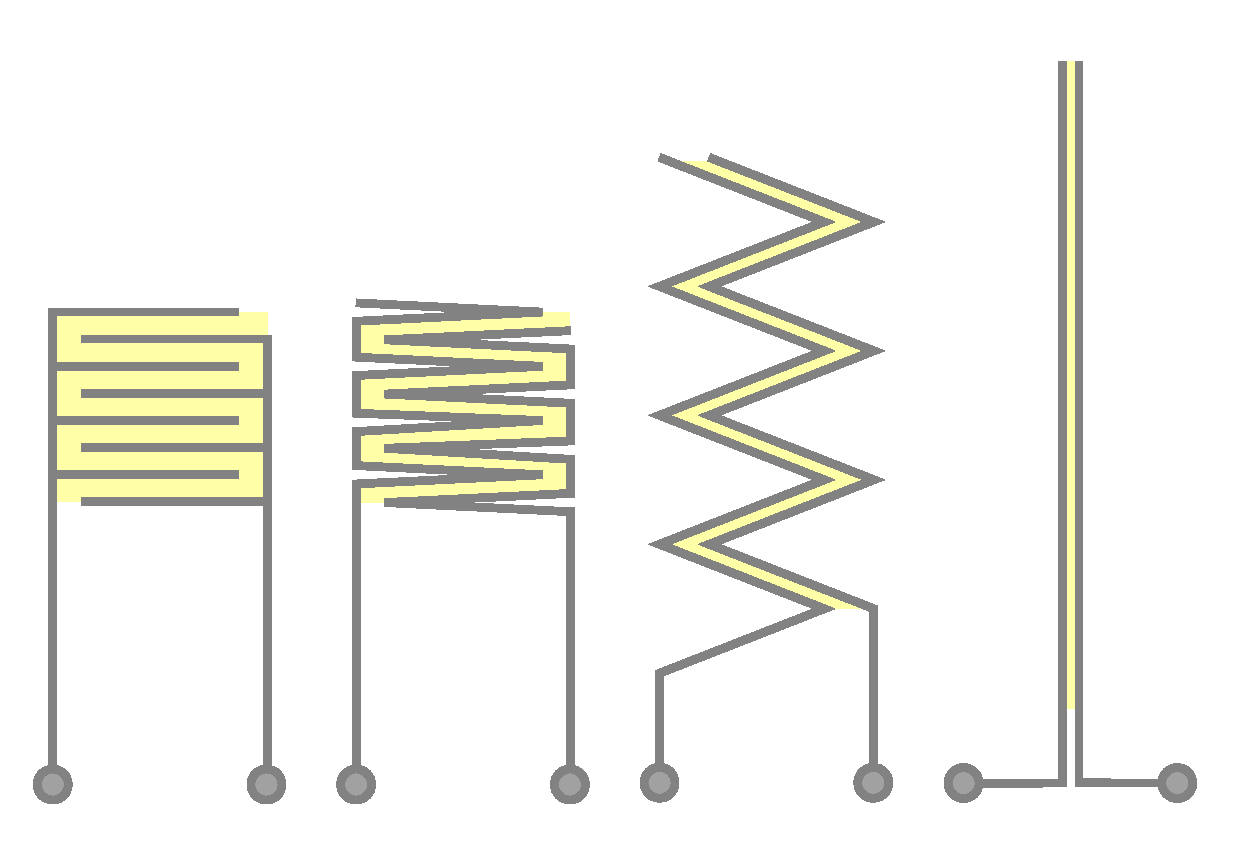
\includegraphics[width=1\textwidth]{./pics_200410/grid.pdf}
       \end{center}
\caption{Transformation of the grid to a line}
     \label{fig:grid}
\end{figure}

The analytic solution of the equation is a tricky, although beautiful problem. Unfortunately I could only obtain numeric solutions for the specific films. I used Comsol for calculations. The problem was brought to a 2D problem with the transformation shown in \ref{fig:grid}. The model in Comsol consists of two copper electrodes (10 $\mu m$ width) and a film (10 $\mu m$ thick, 50 $\mu m$ width). The conductivity of the film was set to $\sigma =\,$1e-2$\,S/cm$. Then three situations were cosidered:
Thick film, where electrodes are thin as compared to the film thickness (1 \% of film thickness): Fig \ref{fig:dits_thick}\\
Intermediate film, where electrodes are of comparable thickness to the film thickness (50 \% of film thickness): Fig\ref{fig:dits_inter}\\
Thin film, where electrodes areas thick as the film(100 \% of film thickness): Fig \ref{fig:dits_thin}\\
 
The calculations show that the current is distributed within the film evenly and it seems like there is no need in using additional models for calculating the conductivity: one can use the bulk formula where electric resistance is an inverse of the conductivity, $R = \frac{1}{\sigma}l/s$, where l is the distance between the fingers and s is the finger's cross-section.

\begin{figure} [!ht]
\begin{center}
       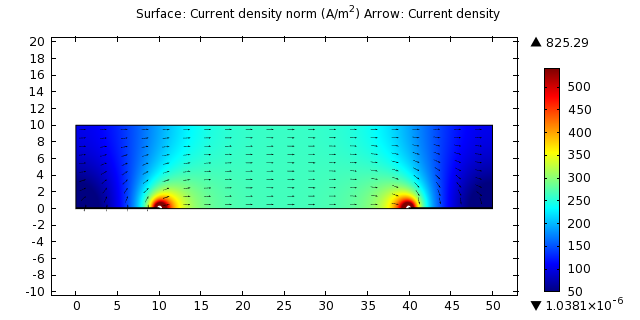
\includegraphics[width=1\textwidth]{./pics_200410/3_thick_film.png}
       \end{center}
\caption{Distribution of electric current in a thick polymer film. The current is uniform in the middle of the film. Let us see, whether we can apply the simple, bulk formula to this structure.}
     \label{fig:dits_thick}
\end{figure}

\begin{figure} [!ht]
\begin{center}
       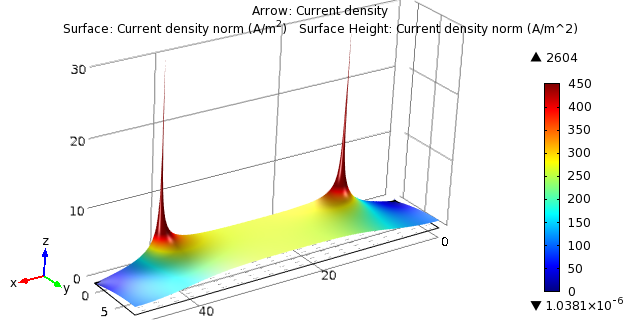
\includegraphics[width=1\textwidth]{./pics_200410/3_thick_film_2.png}
       \end{center}
\caption{Thick film. The current is uniform in the middle of the film. It is better seen on this 3d plot. Let us see, whether we can apply the simple, bulk formula to this structure. I think we do not gain a lot of error by saying that the current is uniform within the whole film.}
     \label{fig:dits_thick}
\end{figure}

\begin{figure} [!ht]
\begin{center}
       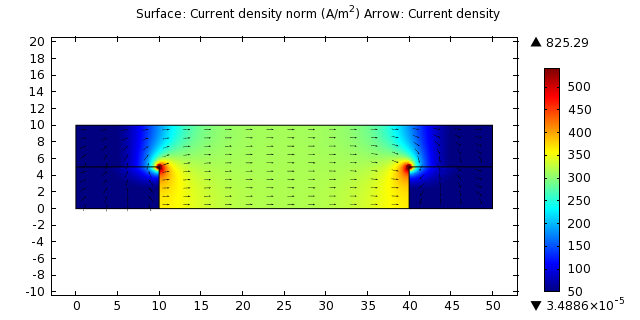
\includegraphics[width=1\textwidth]{./pics_200410/2_intermediate_film.png}
       \end{center}
\caption{Distribution of electric current in an intermediate polymer film}
     \label{fig:dits_inter}
\end{figure}

\begin{figure} [!ht]
\begin{center}
       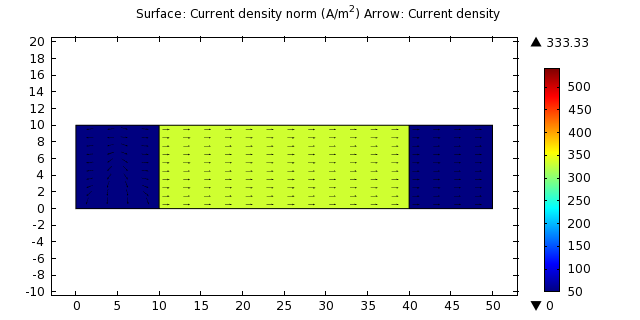
\includegraphics[width=1\textwidth]{./pics_200410/1_thin_film.png}
       \end{center}
\caption{Distribution of electric current in a thin polymer film}
     \label{fig:dits_thin}
\end{figure}

\begin{figure} [!ht]
\begin{center}
       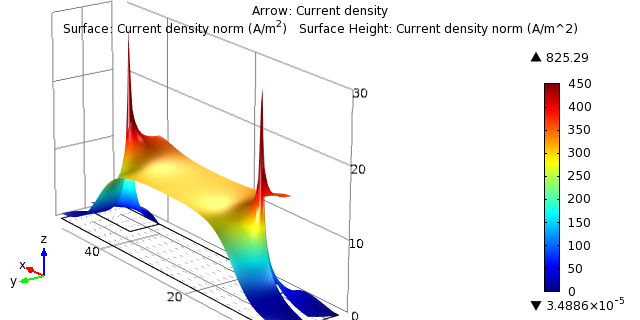
\includegraphics[width=1\textwidth]{./pics_200410/3_intermediate_film_2.png}
       \end{center}
\caption{Very high values of current density in an intermediate film due to the sharp edges of the contacts. This effect might be real.}
     \label{fig:dits_singular}
\end{figure}


\newpage
\section{Next Week}
\paragraph{}
$\bullet$ Five lines in mono-DiTS are interesting. But spin count on the waterfall plots must be done, too.\\
$\bullet$ Writing about the finger grid problem and trying to get quantitative data from Comsol. Precisely, what is the geometric criterion at which one needs to care about the spatial distribution of current? Plan of experiment:\\
1. make a 2d model of film with certain $\sigma$\\
2. apply a fixed potential of 1V to the input terminal, ground the output terminal.
3. measure the total current (still need to figure it out, there are singularities in the current density, as in Fig\ref{fig:dits_singular}.)\\
4. From measured current and applied potential calculate $\sigma$. Use the bulk formula with homogeneous distr. of current density.
5. Change geometry until $\sigma$ is off by 10$\,\%$. Is there a better criterion? Something like 3$\,\sigma$ tolerance for normally distributed values?\\
The numerical solutions show that the current is evenly distributed within the film, if considered far enough from the current terminals. The distance between the terminals should be the parameter that is to vary.


$\bullet$ Continue with restructuring the Hall paper. Last section must be changed. First sections might be too lengthy. When done, let Jan know.\\

%\sectionline{black}{72}

\par A copy of this report as well as other relevant reports are collected in \begin{verbatim}
/net/grouphome/ag-bittl/EPR on Batteries/Writing/report
\end{verbatim} 
%I hope to be back in the institute by Tuesday.

%\newpage
%\begin{thebibliography}{999}
%\bibitem{bib:conformal_mapping} \href{http://www.bru.hlphys.jku.at/conf_map/index.html} {a visualization of electric current flow under a %conformal mapping}. Even Hall effect is considered.
%\bibitem{bib:conformal} \href{https://en.wikipedia.org/wiki/Conformal_map#Physics_and_engineering} {a link to Wikipedia.} Conformal %mapping preserves the laplacian.

%\bibitem{bib:PNDI_mobility} A high-mobility electron-transporting polymer for 
%printed transistors, the Nature paper with FET studies on PNDI
%\bibitem{bib:n-type-doping} n-doping of organic semiconductors, a general review
%\bibitem{p3HT_TOF} TOF mobility measurements in pristine films of P3HT: control of hole
%injection and influence of film thickness
%\bibitem{p3HT_sigmaaldrich} \href{https://www.ossila.com/products/p3ht?_pos=1&_sid=5cb60a34a&_ss=r&variant=18448157343840}{click}
%\bibitem{pBTTT_p3HT_fet} Liquid-crystalline semiconducting polymers with high charge-carrier mobility
%\bibitem{pBTTT_p3HT_structure} Atomic and electronic structure of polymer organic semiconductors: P3HT, PQT, and PBTTT
%\bibitem{DPP-DTT} \href{https://www.ossila.com/products/dpp-dtt-polymer?variant=30366225367136}{clack}
%\bibitem{DPP-DTT_synth} A stable solution-processed polymer semiconductor with record high-mobility for printed transistors

%\end{thebibliography}



\end{document}

